\documentclass[12pt,a4paper]{article}
\usepackage[utf8]{inputenc}
\usepackage[T1]{fontenc}
\usepackage[english]{babel}
\usepackage{geometry}
\usepackage{hyperref}
\usepackage{graphicx}
\usepackage{listings}
\usepackage{xcolor}
\usepackage{booktabs}
\usepackage{tabularx}
\usepackage{array}
\usepackage{caption}
\usepackage{float}
\usepackage{parskip}
\usepackage{enumitem}
\usepackage{titlesec}
\usepackage{subcaption}

\geometry{margin=2.5cm}

\hypersetup{
  colorlinks=true,
  linkcolor=blue!60!black,
  urlcolor=blue!60!black,
  citecolor=blue!60!black
}

\graphicspath{{diagrams/}}

\definecolor{codegray}{rgb}{0.95,0.95,0.95}
\definecolor{codecomment}{rgb}{0.4,0.4,0.4}
\definecolor{codekeyword}{rgb}{0.0,0.3,0.7}
\definecolor{codestring}{rgb}{0.2,0.5,0.2}
\definecolor{codeannotation}{rgb}{0.6,0.3,0.0}
\definecolor{codered}{RGB}{180,30,30}
\definecolor{codegreen}{RGB}{0,120,0}
\definecolor{warnorange}{RGB}{200,100,0}
\definecolor{diffadd}{RGB}{0,100,0}
\definecolor{diffrem}{RGB}{180,30,30}

\lstset{
  language=Java,
  backgroundcolor=\color{codegray},
  basicstyle=\ttfamily\small,
  keywordstyle=\color{codekeyword}\bfseries,
  commentstyle=\color{codecomment}\itshape,
  stringstyle=\color{codestring},
  numbers=left,
  numberstyle=\tiny\color{gray},
  numbersep=8pt,
  breaklines=true,
  showstringspaces=false,
  frame=single,
  framerule=0pt,
  xleftmargin=1em,
  xrightmargin=0.5em,
  captionpos=b,
  extendedchars=true,
}

\newcommand{\code}[1]{\texttt{#1}}
\newcommand{\cls}[1]{\texttt{#1}}
\newcommand{\meth}[1]{\texttt{#1}}
\newcommand{\pkg}[1]{\texttt{#1}}
\newcommand{\file}[1]{\texttt{#1}}
\newcommand{\removed}[1]{\textcolor{diffrem}{\sout{#1}}}
\newcommand{\added}[1]{\textcolor{diffadd}{\textbf{#1}}}

\title{GUI Refactoring Changelog \\
       \large \texttt{org.openmarkov.gui} --- Applied Changes}
\author{OpenMarkov --- CISIAD, UNED}
\date{April 2026}

\begin{document}

\maketitle
\tableofcontents
\newpage

% ===================================================================
\section{Overview}
\label{sec:overview}
% ===================================================================

This document records the refactoring changes applied to the
\pkg{org.openmarkov.gui} module as part of the GUI improvement plan
described in \file{refactorizacion-gui.tex}. Each section covers one
refactoring, showing the state before and after the change, the
motivation, and the files affected.

\begin{table}[H]
\centering
\small
\begin{tabular}{llll}
\toprule
\textbf{Ref.} & \textbf{Description} & \textbf{Date} & \textbf{Status} \\
\midrule
R3 & Eliminate unsafe \cls{TablePotential} casts & April 2026 & Done \\
R5 & Consolidate CPT value-edit duplication       & April 2026 & Done \\
R8 & Consolidate temporal interval editors        & April 2026 & Discarded \\
\bottomrule
\end{tabular}
\caption{Refactoring entries in this changelog.}
\label{tab:overview}
\end{table}

% ===================================================================
\section{R3 --- Elimination of Unsafe Casts to TablePotential}
\label{sec:r3}
% ===================================================================

% -------------------------------------------------------------------
\subsection{Motivation}
% -------------------------------------------------------------------

The GUI module contained 16 explicit casts to \cls{TablePotential} and
10 \code{instanceof TablePotential} checks. Most of them originated
from \meth{Link.getRestrictionsPotential()}, which returned
\cls{Potential} (the abstract base type) even though the underlying
field was already declared as \cls{TablePotential}. This forced every
caller to cast, hiding potential \code{NullPointerException} errors
and cluttering the code with redundant type assertions.

% -------------------------------------------------------------------
\subsection{Before}
% -------------------------------------------------------------------

\begin{figure}[H]
\centering
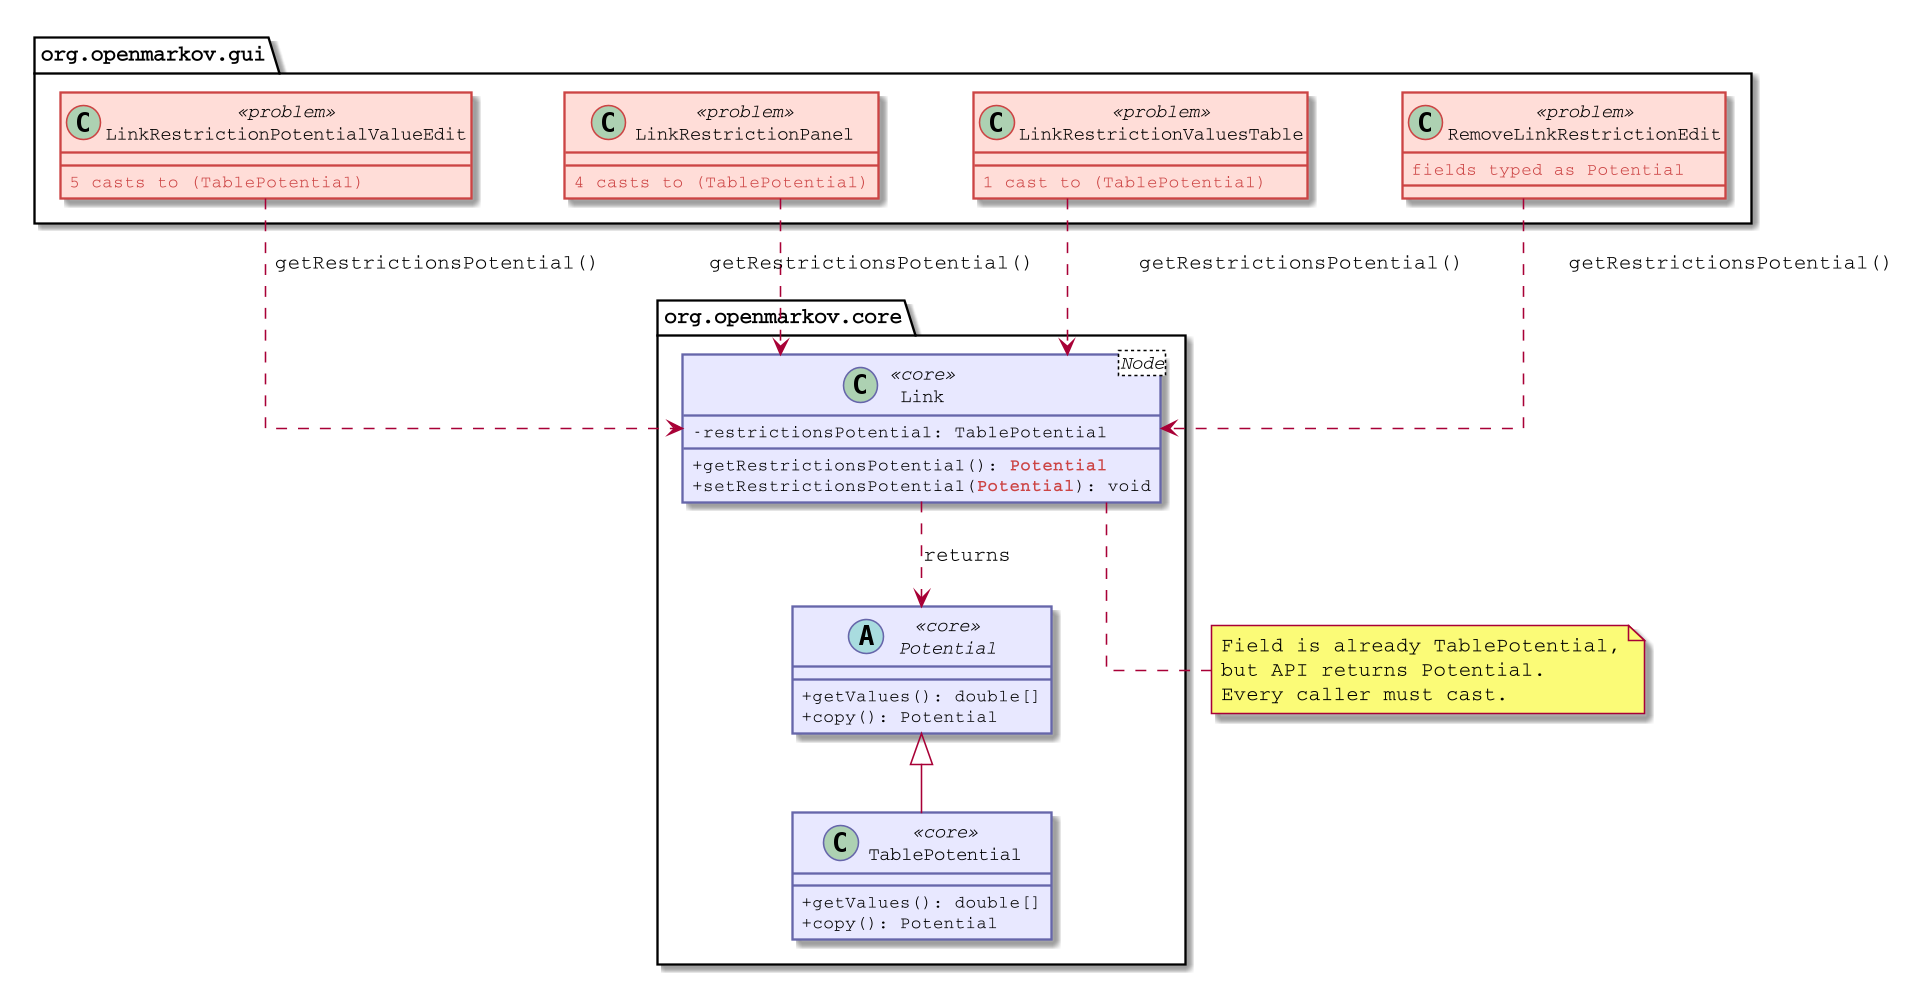
\includegraphics[width=0.85\textwidth]{r3-before.png}
\caption{Before R3: \cls{Link} exposes \cls{Potential} in its API.
         Every GUI caller must cast to \cls{TablePotential}.
         Diagram source: \file{r3-before.puml}.}
\label{fig:r3-before}
\end{figure}

The getter and setter signatures in \cls{Link.java} were:

\begin{lstlisting}[caption={Link.java --- before R3}]
// Field is already TablePotential
private TablePotential restrictionsPotential;

// But the API returns the abstract type
public Potential getRestrictionsPotential() {
    return restrictionsPotential;
}

public void setRestrictionsPotential(Potential potential) {
    this.restrictionsPotential = (TablePotential) potential;
}
\end{lstlisting}

This forced callers to write unsafe casts like:

\begin{lstlisting}[caption={Typical caller code --- before R3}]
TablePotential tp =
    (TablePotential) link.getRestrictionsPotential();
\end{lstlisting}

Additionally, classes like \cls{TablePotentialValueEdit} used the
legacy check-then-cast pattern:

\begin{lstlisting}[caption={Check-then-cast pattern --- before R3}]
this.isExactDistrPotential =
    potential instanceof ExactDistrPotential;
if (getExactDistrPotential()) {
    this.oldExactDistrPotential =
        (ExactDistrPotential) potential;
    this.oldTablePotential =
        ((ExactDistrPotential) potential).getTablePotential();
} else {
    this.oldTablePotential = (TablePotential) potential;
}
\end{lstlisting}

% -------------------------------------------------------------------
\subsection{After}
% -------------------------------------------------------------------

\begin{figure}[H]
\centering
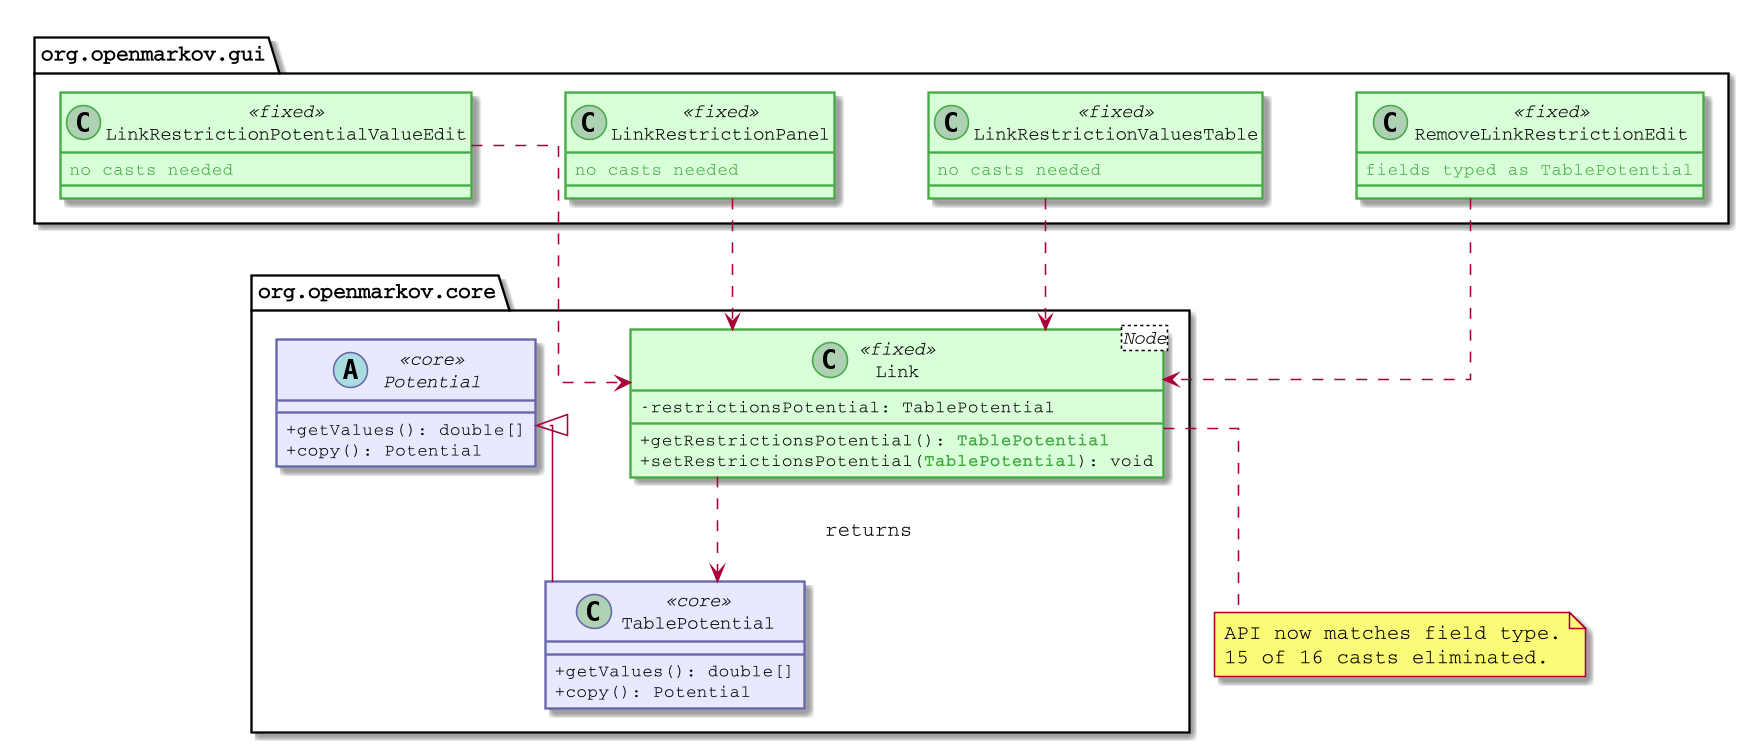
\includegraphics[width=0.85\textwidth]{r3-after.png}
\caption{After R3: \cls{Link} returns \cls{TablePotential} directly.
         No casts needed in GUI callers.
         Diagram source: \file{r3-after.puml}.}
\label{fig:r3-after}
\end{figure}

\subsubsection{Change 1: Typed getter and setter in Link.java}

\begin{lstlisting}[caption={Link.java --- after R3}]
private TablePotential restrictionsPotential;

public TablePotential getRestrictionsPotential() {
    return restrictionsPotential;
}

public void setRestrictionsPotential(TablePotential potential) {
    this.restrictionsPotential = potential;
}
\end{lstlisting}

This single change eliminated 10 casts across 4 GUI classes:
\cls{LinkRestrictionPotentialValueEdit} (5),
\cls{LinkRestrictionPanel} (4),
\cls{LinkRestrictionValuesTable} (1).

\subsubsection{Change 2: Pattern matching instanceof (Java~21)}

The check-then-cast pattern was replaced with Java~21 pattern matching:

\begin{lstlisting}[caption={Pattern matching instanceof --- after R3}]
if (potential instanceof ExactDistrPotential exactDistr) {
    this.oldExactDistrPotential = exactDistr;
    this.oldTablePotential =
        exactDistr.getTablePotential();
} else if (potential instanceof TablePotential table) {
    this.oldTablePotential = table;
}
\end{lstlisting}

\begin{figure}[H]
\centering
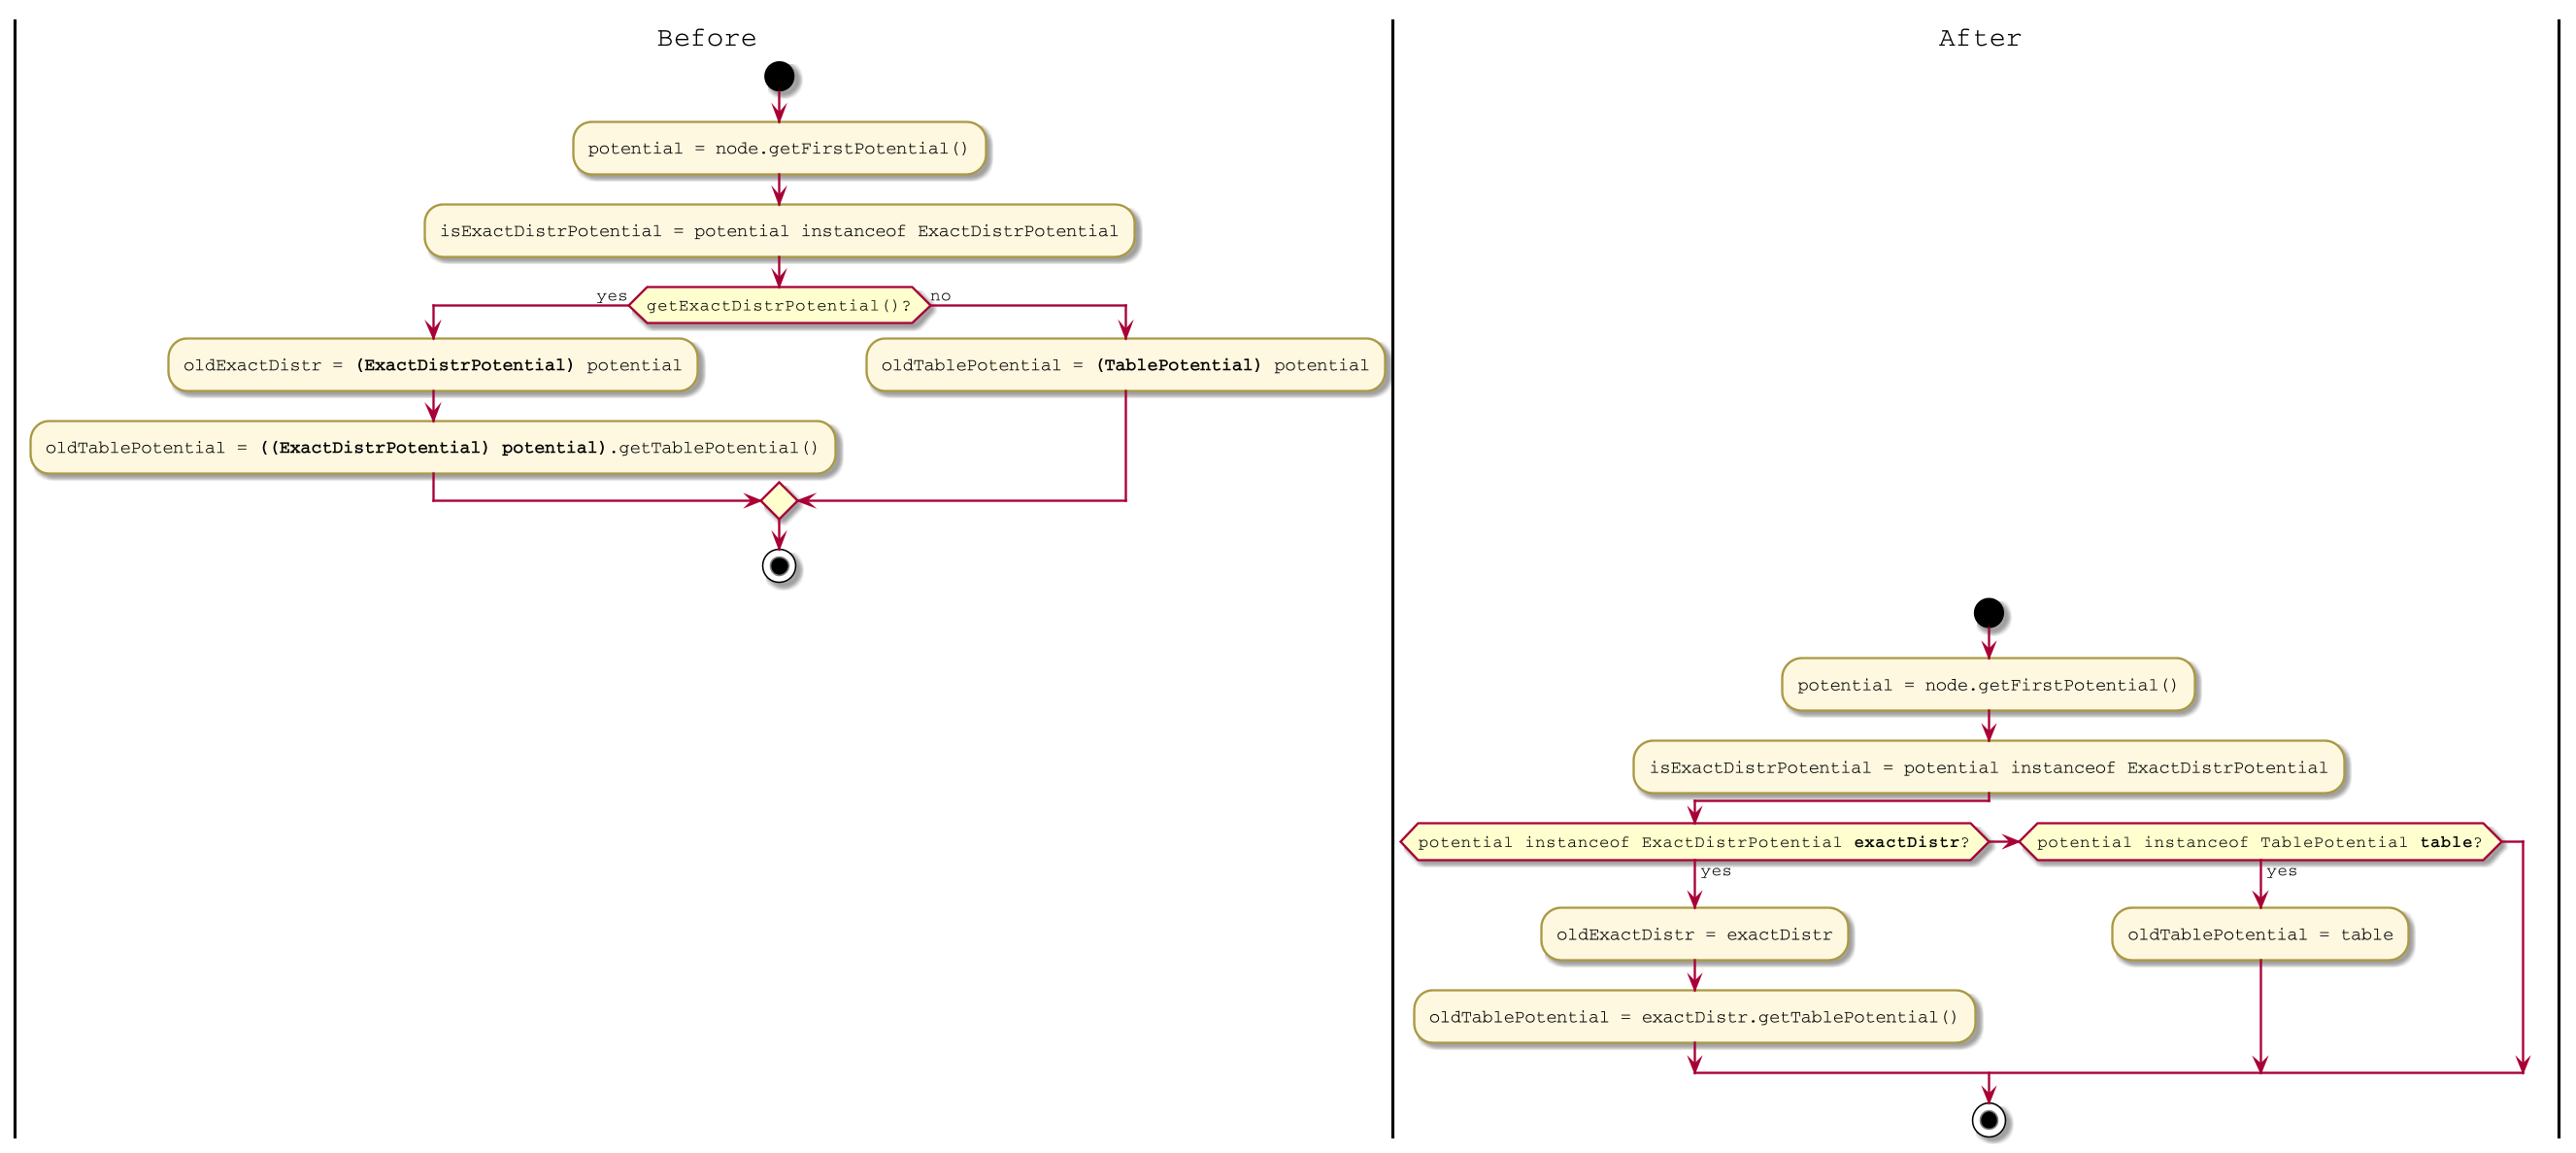
\includegraphics[width=0.7\textwidth]{r3-instanceof.png}
\caption{Flow comparison: legacy check-then-cast vs.\ pattern matching
         \code{instanceof}. Diagram source: \file{r3-instanceof.puml}.}
\label{fig:r3-instanceof}
\end{figure}

This was applied in:
\begin{itemize}[nosep]
  \item \cls{TablePotentialValueEdit} --- constructor
  \item \cls{TablePotentialPanel} --- ternary expression
  \item \cls{ValuesTable} --- potential type dispatch
  \item \cls{PotentialsTablePanelOperations} --- exact distribution
        check
\end{itemize}

\subsubsection{Change 3: Null safety in ProbNetCopier}

The \meth{getNode()} method in \cls{ProbNet} can return \code{null}.
Three calls in \cls{ProbNetCopier} assumed the node would always be
found (because it was cloned immediately before). We wrapped them with
\meth{Objects.requireNonNull()} to make the invariant explicit:

\begin{lstlisting}[caption={ProbNetCopier.java --- null safety}]
Objects.requireNonNull(
    dest.getNode(node.getName()),
    "Node not found in dest: " + node.getName()
).setPotentials(newPotentials);
\end{lstlisting}

% -------------------------------------------------------------------
\subsection{Summary of impact}
% -------------------------------------------------------------------

\begin{table}[H]
\centering
\small
\begin{tabular}{lrl}
\toprule
\textbf{File} & \textbf{Casts removed} & \textbf{Method} \\
\midrule
Link.java (core)                      & 1 (internal) & Typed getter/setter \\
LinkRestrictionPotentialValueEdit      & 5 & No longer needed \\
LinkRestrictionPanel                   & 4 & No longer needed \\
LinkRestrictionValuesTable             & 1 & No longer needed \\
RemoveLinkRestrictionEdit              & 0 & Fields retyped \\
TablePotentialValueEdit                & 1 of 3 & Pattern matching \\
TablePotentialPanel                    & 1 & Pattern matching \\
ValuesTable                            & 1 & Pattern matching \\
PotentialsTablePanelOperations         & 1 & Pattern matching \\
\midrule
\textbf{Total}                         & \textbf{15 of 16} & 1 cast remains \\
\bottomrule
\end{tabular}
\caption{R3 impact per file.}
\label{tab:r3-impact}
\end{table}

The single remaining cast is in \cls{PotentialsTablePanelOperations},
where \meth{Potential.copy()} returns \cls{Potential} (the base type).
This is inherent to the API and cannot be removed without a covariant
return type on \meth{copy()}.


% ===================================================================
\section{R5 --- Consolidation of CPT Value-Edit Duplication}
\label{sec:r5}
% ===================================================================

% -------------------------------------------------------------------
\subsection{Motivation}
% -------------------------------------------------------------------

The probability redistribution algorithm---given an array of values
and a priority list, adjust the values so they sum to~1.0---was
duplicated three times across two classes:

\begin{enumerate}[nosep]
  \item \cls{TablePotentialValueEdit} constructor (1 copy, $\sim$40
        lines)
  \item \cls{ICITablePotentialValueEdit.doEdit()} --- leaky parameters
        ($\sim$35 lines)
  \item \cls{ICITablePotentialValueEdit.doEdit()} --- noisy parameters
        ($\sim$35 lines, identical to leaky)
\end{enumerate}

% -------------------------------------------------------------------
\subsection{Before}
% -------------------------------------------------------------------

\begin{figure}[H]
\centering
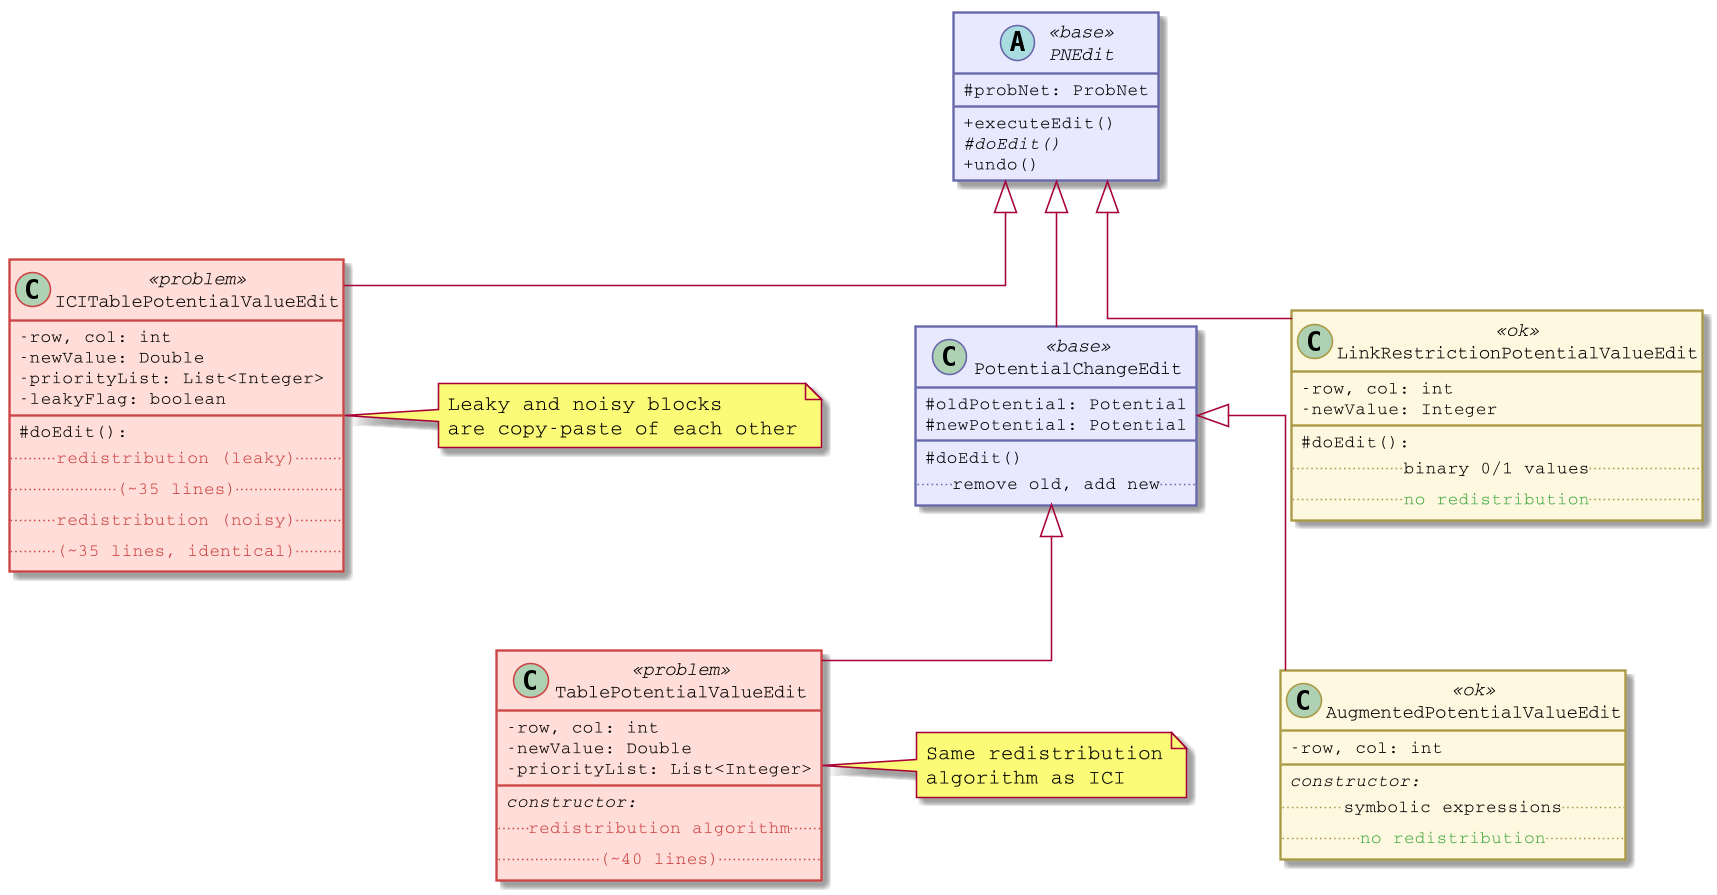
\includegraphics[width=0.95\textwidth]{r5-before.png}
\caption{Before R5: the redistribution algorithm is duplicated in
         \cls{TablePotentialValueEdit} and twice in
         \cls{ICITablePotentialValueEdit}.
         Diagram source: \file{r5-before.puml}.}
\label{fig:r5-before}
\end{figure}

The redistribution in \cls{TablePotentialValueEdit} (constructor):

\begin{lstlisting}[caption={TablePotentialValueEdit --- before R5 (abbreviated)}]
// ~40 lines in the constructor
Iterator<Integer> listIterator = priorityList.listIterator();
double sum = 0.0;
int maxDecimals = 10;
double epsilon = Math.pow(10, -(maxDecimals + 2));
newTable[potentialSelected] =
    Util.roundAndReduce(newValue, epsilon, maxDecimals);
while (listIterator.hasNext()) {
    position = listIterator.next();
    if (isEditablePosition(position)) {
        sum = Util.roundAndReduce(
            sum + newTable[position], epsilon, maxDecimals);
    }
}
double rest = Math.abs(
    Util.roundAndReduce(1 - sum, epsilon, maxDecimals));
if (sum > 1.0) {
    // subtract from cells in priority order ...
} else {
    // add remainder to first editable cell ...
}
\end{lstlisting}

In \cls{ICITablePotentialValueEdit.doEdit()}, the same algorithm
appeared twice---once for leaky parameters and once for noisy
parameters---with only the array name changing:

\begin{lstlisting}[caption={ICITablePotentialValueEdit.doEdit() --- before R5 (abbreviated)}]
if (leakyFlag) {
    // ~35 lines: redistribute newLeakyParameters
    newLeakyParameters[position] = Util.roundAndReduce(...);
    // ... sum, rest, redistribute loop ...
    iciPotentialEdit = new ICIPotentialEdit(
        probNet, iciPotential, newLeakyParameters);
} else {
    // ~35 lines: redistribute newNoisyParameters (identical logic)
    newNoisyParameters[position] = Util.roundAndReduce(...);
    // ... sum, rest, redistribute loop ...
    iciPotentialEdit = new ICIPotentialEdit(
        probNet, iciPotential, noisyVariable, newNoisyParameters);
}
\end{lstlisting}

% -------------------------------------------------------------------
\subsection{After}
% -------------------------------------------------------------------

\begin{figure}[H]
\centering
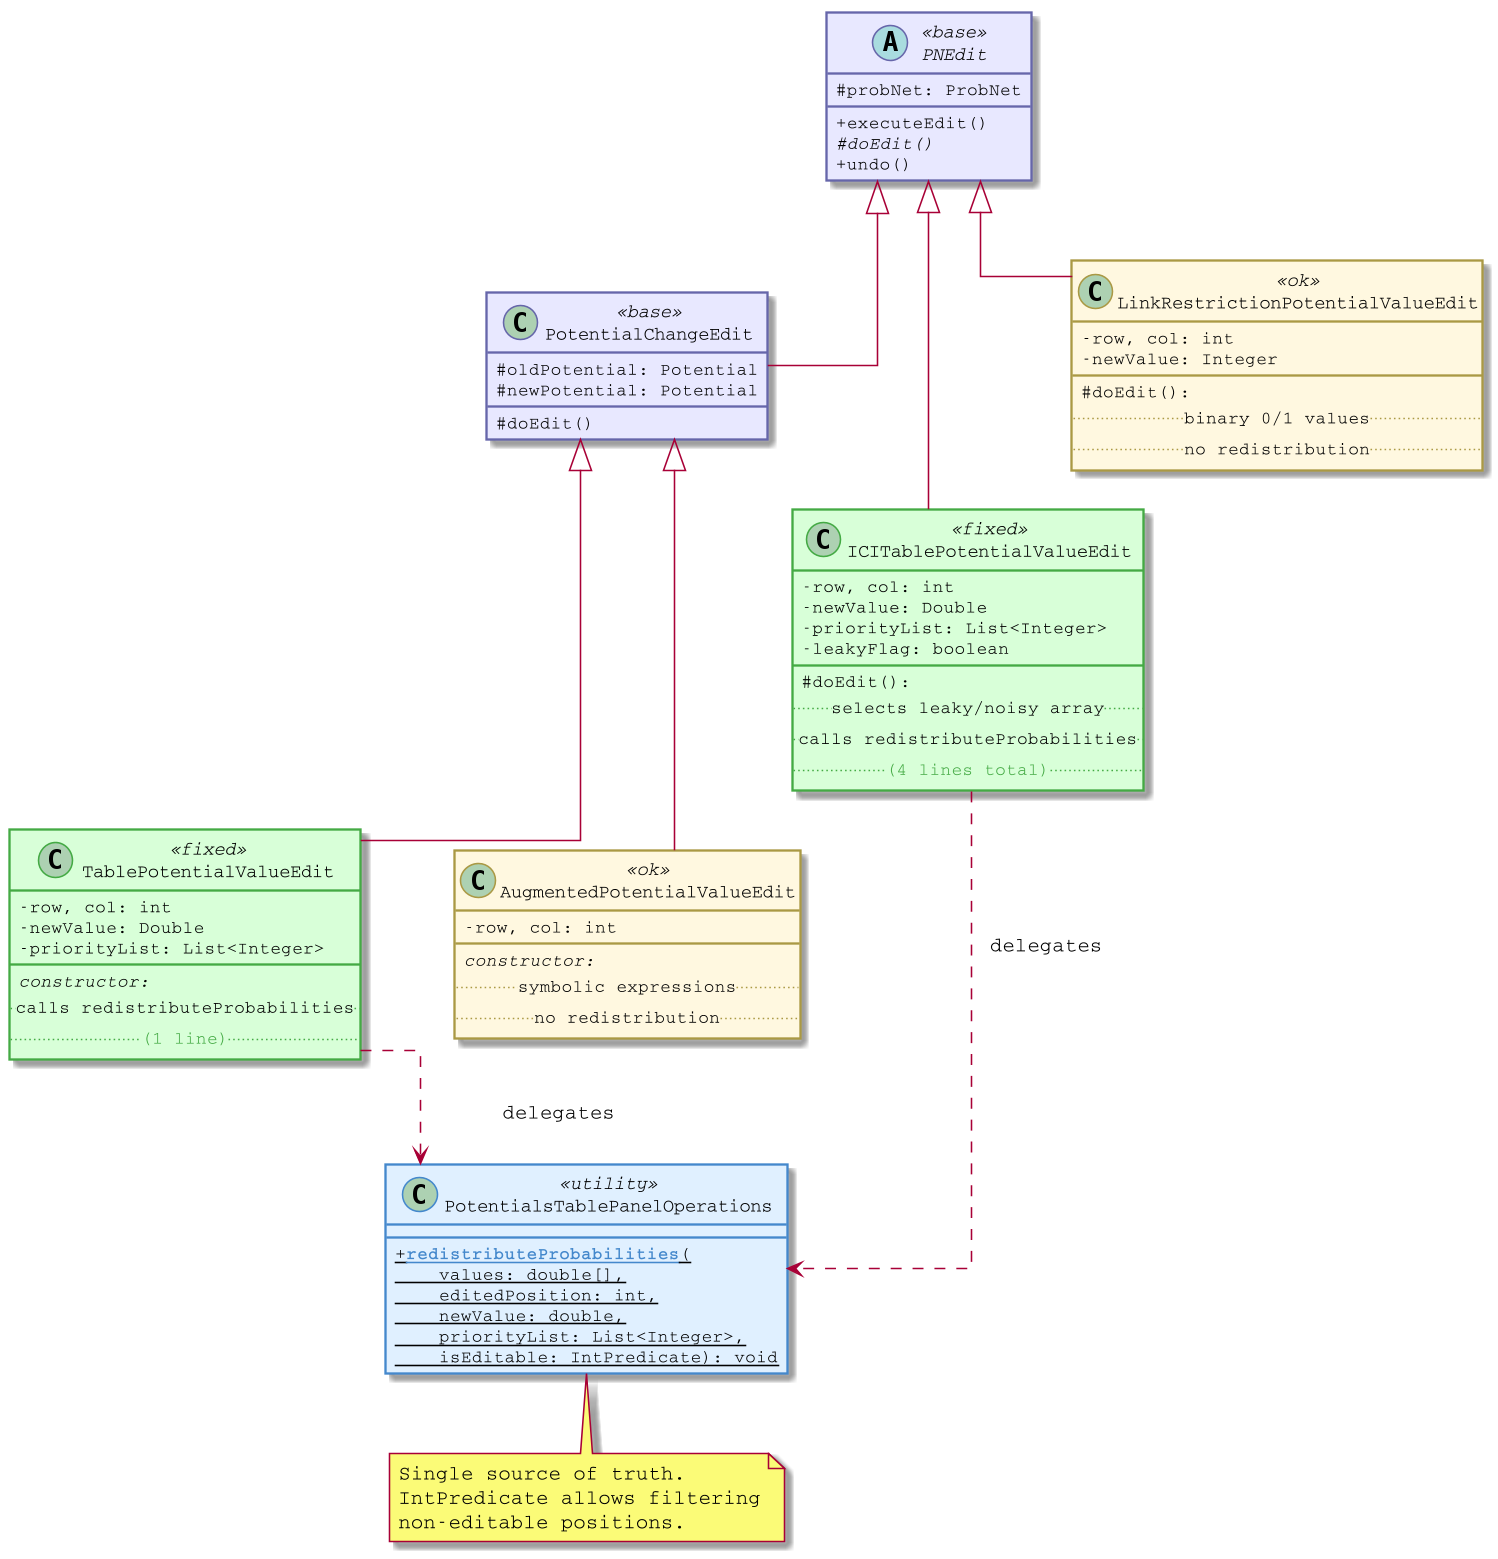
\includegraphics[width=0.95\textwidth]{r5-after.png}
\caption{After R5: both classes delegate to a single
         \meth{redistributeProbabilities()} method in
         \cls{PotentialsTablePanelOperations}.
         Diagram source: \file{r5-after.puml}.}
\label{fig:r5-after}
\end{figure}

\subsubsection{New utility method}

The algorithm was extracted to a static method in
\cls{PotentialsTablePanelOperations}, which was already a utility
class for table potential operations:

\begin{lstlisting}[caption={PotentialsTablePanelOperations.redistributeProbabilities()}]
public static void redistributeProbabilities(
        double[] values,
        int editedPosition,
        double newValue,
        List<Integer> priorityList,
        IntPredicate isEditable) {
    int maxDecimals = 10;
    double epsilon = Math.pow(10, -(maxDecimals + 2));
    values[editedPosition] =
        Util.roundAndReduce(newValue, epsilon, maxDecimals);

    double sum = 0.0;
    for (int pos : priorityList) {
        if (isEditable.test(pos)) {
            sum = Util.roundAndReduce(
                sum + values[pos], epsilon, maxDecimals);
        }
    }

    double rest = Math.abs(
        Util.roundAndReduce(1 - sum, epsilon, maxDecimals));
    if (sum > 1.0) {
        for (int pos : priorityList) {
            if (rest == 0) break;
            if (isEditable.test(pos)) {
                rest = Util.roundAndReduce(
                    rest - values[pos], epsilon, maxDecimals);
                if (rest < 0) {
                    values[pos] = Math.abs(
                        Util.roundAndReduce(rest, epsilon, maxDecimals));
                    break;
                }
                values[pos] = 0.0;
            }
        }
    } else {
        for (int pos : priorityList) {
            if (isEditable.test(pos)) {
                values[pos] = Util.roundAndReduce(
                    values[pos] + rest, epsilon, maxDecimals);
                break;
            }
        }
    }
}
\end{lstlisting}

The \code{IntPredicate isEditable} parameter is the key design
decision: \cls{TablePotentialValueEdit} passes a method reference
\code{this::isEditablePosition} to filter non-editable cells, while
\cls{ICITablePotentialValueEdit} passes \code{pos -> true} because
all ICI parameter positions are always editable.

\begin{figure}[H]
\centering
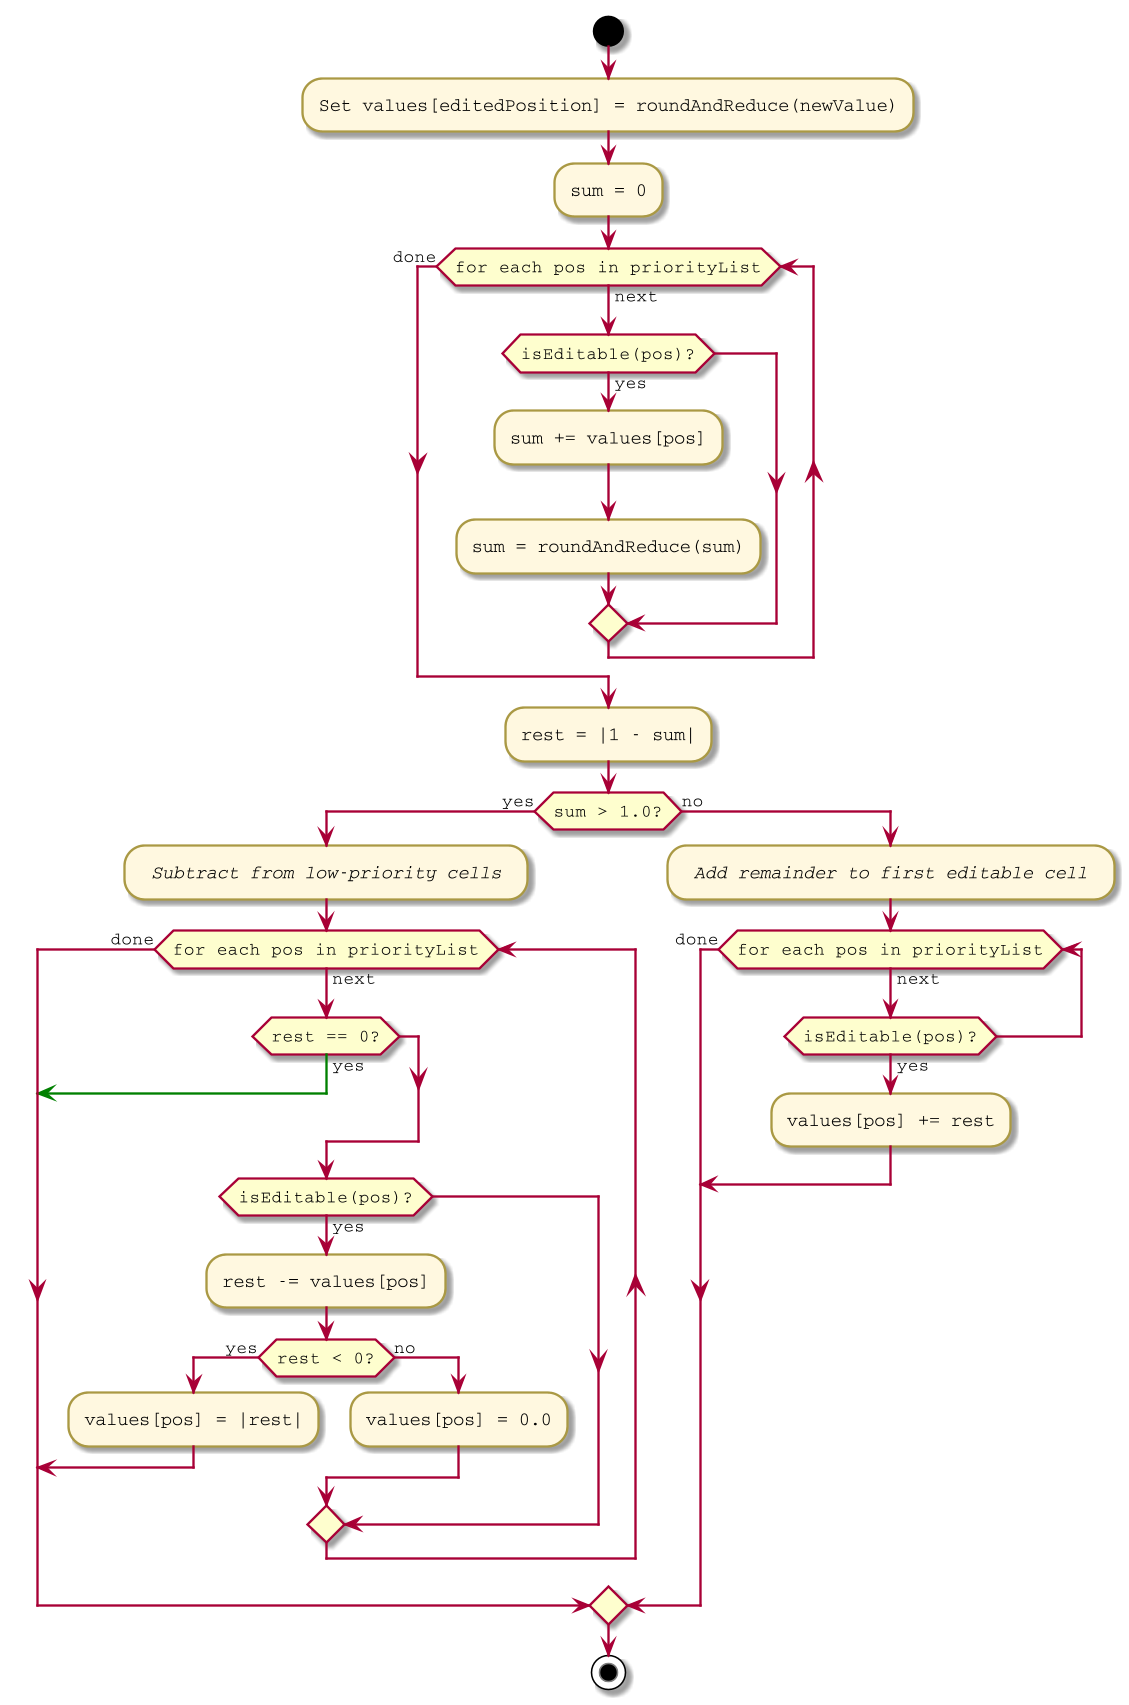
\includegraphics[width=0.55\textwidth]{r5-algorithm.png}
\caption{Flowchart of the redistribution algorithm.
         Diagram source: \file{r5-algorithm.puml}.}
\label{fig:r5-algorithm}
\end{figure}

\subsubsection{Simplified callers}

\cls{TablePotentialValueEdit} constructor (was $\sim$40 lines):

\begin{lstlisting}[caption={TablePotentialValueEdit --- after R5}]
PotentialsTablePanelOperations.redistributeProbabilities(
    newTable, potentialSelected, newValue,
    priorityList, this::isEditablePosition);
\end{lstlisting}

\cls{ICITablePotentialValueEdit.doEdit()} (was $\sim$70 lines):

\begin{lstlisting}[caption={ICITablePotentialValueEdit.doEdit() --- after R5}]
double[] params = leakyFlag
    ? newLeakyParameters : newNoisyParameters;
PotentialsTablePanelOperations.redistributeProbabilities(
    params, position, newValue, priorityList, pos -> true);

ICIPotentialEdit iciPotentialEdit = leakyFlag
    ? new ICIPotentialEdit(probNet, iciPotential,
                           newLeakyParameters)
    : new ICIPotentialEdit(probNet, iciPotential,
                           noisyVariable, newNoisyParameters);
iciPotentialEdit.executeEdit();
\end{lstlisting}

% -------------------------------------------------------------------
\subsection{Design rationale}
% -------------------------------------------------------------------

The four CPT value-editing classes use two incompatible inheritance
trees (\cls{PotentialChangeEdit} vs.\ \cls{PNEdit} directly), different
value types (double, symbolic, binary), and different execution models
(constructor vs.\ \meth{doEdit()}). A common base class would have
required restructuring the entire edit hierarchy for little gain.

Extracting the shared \emph{algorithm} (redistribution) into a static
utility method, parameterized with an \code{IntPredicate} for
editability, was the simplest approach that eliminated the duplication
without touching the class hierarchy.

% -------------------------------------------------------------------
\subsection{Summary of impact}
% -------------------------------------------------------------------

\begin{table}[H]
\centering
\small
\begin{tabular}{lrrl}
\toprule
\textbf{File} & \textbf{Lines removed} & \textbf{Lines added} & \textbf{Change} \\
\midrule
PotentialsTablePanelOperations  & 0  & 30 & New utility method \\
TablePotentialValueEdit         & 40 & 2  & Delegates to utility \\
ICITablePotentialValueEdit      & 70 & 6  & Delegates to utility \\
\midrule
\textbf{Net}                    & \multicolumn{2}{c}{\textbf{$-$72 lines}} & \\
\bottomrule
\end{tabular}
\caption{R5 impact per file.}
\label{tab:r5-impact}
\end{table}


% ===================================================================
\section{R8 --- Temporal Interval Editors (Discarded)}
\label{sec:r8}
% ===================================================================

% -------------------------------------------------------------------
\subsection{Analysis and decision}
% -------------------------------------------------------------------

Three interval-editing classes were analyzed for possible
consolidation:

\begin{table}[H]
\centering
\small
\begin{tabular}{lr}
\toprule
\textbf{Class} & \textbf{Lines} \\
\midrule
\cls{NodePartitionedIntervalEdit}   & 165 \\
\cls{RevelationIntervalEdit}        & 152 \\
\cls{PartitionedIntervalEdit}       & 47  \\
\midrule
\textbf{Total}                      & \textbf{364} \\
\bottomrule
\end{tabular}
\caption{R8 candidate classes.}
\label{tab:r8-classes}
\end{table}

The refactoring was discarded because the three classes do not share
enough structure to justify a common abstraction:

\begin{enumerate}
  \item \textbf{Different operation models}:
    \cls{PartitionedIntervalEdit} (47~lines) performs a wholesale
    replacement; \cls{NodePartitionedIntervalEdit} modifies properties
    in place; \cls{RevelationIntervalEdit} manages a list of
    intervals on a link (add, remove, modify, toggle).

  \item \textbf{Incompatible action sets}:
    0, 2, and 4~actions respectively---no common interface.

  \item \textbf{Different backup strategies}:
    scalar \code{double}, object reference, or both.

  \item \textbf{Low volume}: 364~lines with only partial overlap
        does not justify the maintenance cost of an abstraction.
\end{enumerate}

% ===================================================================
\section{R4 --- MainMenu Simplification}
\label{sec:r4}
% ===================================================================

% -------------------------------------------------------------------
\subsection{Problem}
% -------------------------------------------------------------------

\cls{MainMenu} (1,529 lines) declared \textbf{53 fields} of type
\code{JMenu}/\code{JMenuItem}/\code{JCheckBoxMenuItem} and constructed
them via \textbf{46 lazy-getter methods}, each following an identical
pattern:

\begin{lstlisting}[caption={Typical lazy-getter pattern (repeated 46 times)}]
private JMenuItem getFileNewMenuItem() {
    if (fileNewMenuItem == null) {
        fileNewMenuItem = new LocalizedMenuItem(
            MenuItemNames.FILE_NEW,
            ActionCommands.NEW_NETWORK.getCommandName());
        fileNewMenuItem.setIcon(IconBind.NEW_ENABLED.icon());
        fileNewMenuItem.setAccelerator(
            KeyStroke.getKeyStroke(KeyEvent.VK_N, CTRL));
        fileNewMenuItem.addActionListener(listener);
    }
    return fileNewMenuItem;
}
\end{lstlisting}

Additionally, \cls{MainPanelMenuAssistant} accessed items through a
\textbf{43-case switch} in \meth{getJComponentActionCommand()}.

The problems were:
\begin{enumerate}
  \item \textbf{Massive repetition}: 53 fields and 46 getters with
        identical structure.
  \item \textbf{Maintenance cost}: adding a menu item required a field
        declaration, a lazy getter, adding to the parent menu, and
        registering in \cls{MenuItemNames}.
  \item \textbf{Size}: 1,529 lines made navigation difficult.
  \item \textbf{Fragile switch}: the 43-case switch had to be kept in
        sync with the fields manually.
\end{enumerate}

% -------------------------------------------------------------------
\subsection{Before}
% -------------------------------------------------------------------

\begin{figure}[H]
\centering
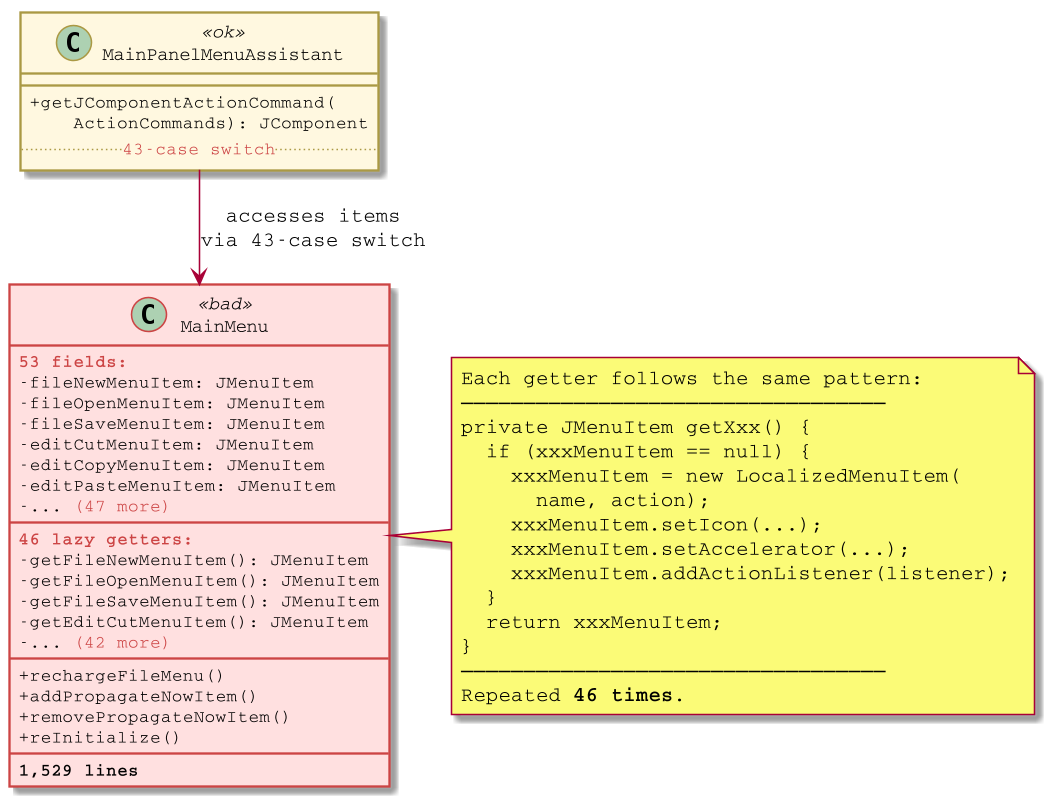
\includegraphics[width=0.85\textwidth]{r4-before.png}
\caption{Before R4: 53 fields, 46 lazy getters, and a 43-case switch
         for item lookup. Diagram source: \file{r4-before.puml}.}
\label{fig:r4-before}
\end{figure}

% -------------------------------------------------------------------
\subsection{After}
% -------------------------------------------------------------------

\begin{figure}[H]
\centering
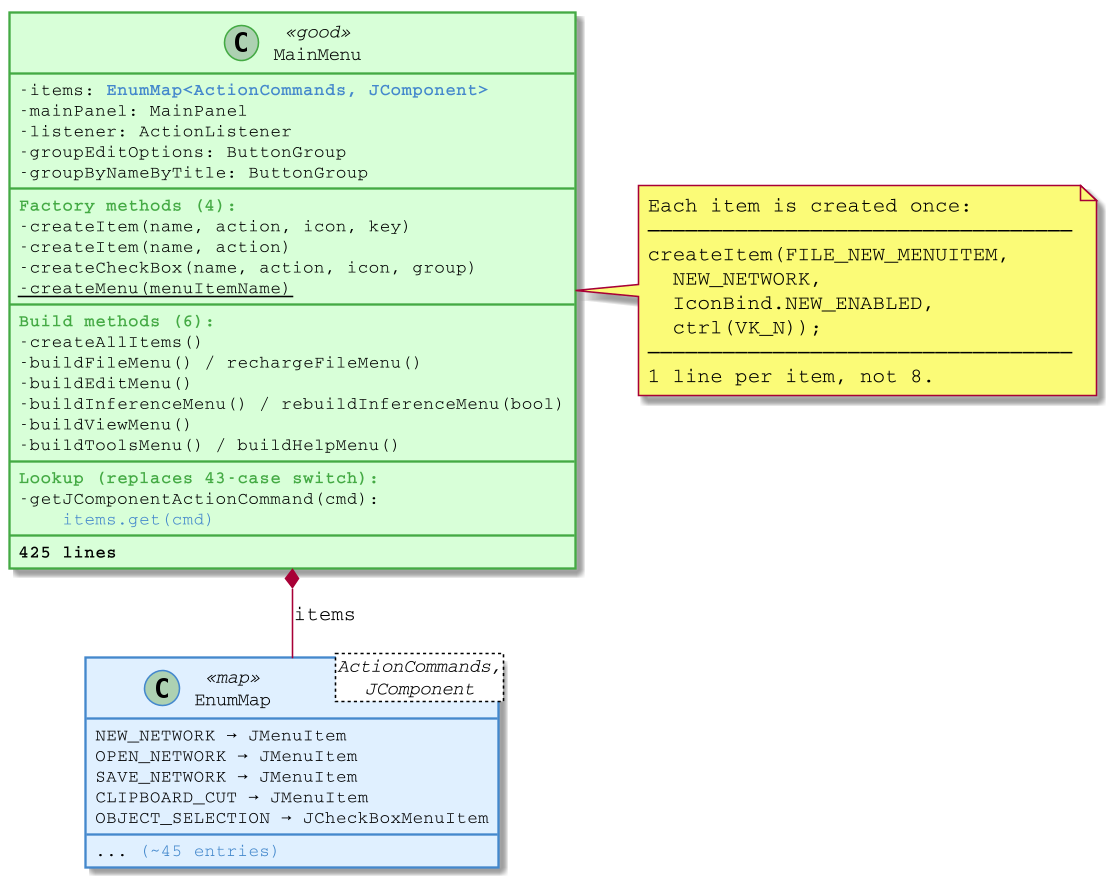
\includegraphics[width=0.85\textwidth]{r4-after.png}
\caption{After R4: all items stored in an \code{EnumMap}, created via
         factory methods. Diagram source: \file{r4-after.puml}.}
\label{fig:r4-after}
\end{figure}

The rewrite introduced four key changes:

\subsubsection{EnumMap replaces 53 fields}

All menu items are stored in a single map:
\begin{lstlisting}[caption={Central item storage}]
private final Map<ActionCommands, JComponent> items =
    new EnumMap<>(ActionCommands.class);
\end{lstlisting}

\subsubsection{Factory methods replace 46 lazy getters}

Two factory methods create items and register them in the map:
\begin{lstlisting}[caption={Factory methods (replacing 46 lazy getters)}]
private void createItem(String name, ActionCommands action,
                        IconBind icon, KeyStroke key) {
    var item = new LocalizedMenuItem(
        name, action.getCommandName(), icon, key);
    item.addActionListener(listener);
    items.put(action, item);
}

private void createCheckBox(String name, ActionCommands action,
                             IconBind icon, ButtonGroup group) {
    var item = icon != null
        ? new LocalizedCheckBoxMenuItem(name, action.getCommandName(), icon)
        : new LocalizedCheckBoxMenuItem(name, action.getCommandName());
    item.addActionListener(listener);
    if (group != null) group.add(item);
    items.put(action, item);
}
\end{lstlisting}

All items are created once in \meth{createAllItems()}, with one line
per item instead of eight:
\begin{lstlisting}[caption={Declarative item creation (excerpt)}]
createItem(FILE_NEW_MENUITEM,  NEW_NETWORK,  NEW_ENABLED,  ctrl(VK_N));
createItem(FILE_OPEN_MENUITEM, OPEN_NETWORK, OPEN_ENABLED, ctrl(VK_O));
createItem(FILE_SAVE_MENUITEM, SAVE_NETWORK, SAVE_ENABLED, ctrl(VK_S));
\end{lstlisting}

\subsubsection{Build methods replace imperative construction}

Menu population reads like a declarative spec:
\begin{lstlisting}[caption={Menu builder (example: Edit menu)}]
private JMenu buildEditMenu() {
    editMenu = createMenu(MenuItemNames.EDIT_MENU);
    editMenu.add(items.get(ActionCommands.CLIPBOARD_CUT));
    editMenu.add(items.get(ActionCommands.CLIPBOARD_COPY));
    editMenu.add(items.get(ActionCommands.CLIPBOARD_PASTE));
    editMenu.add(items.get(ActionCommands.OBJECT_REMOVAL));
    editMenu.addSeparator();
    editMenu.add(items.get(ActionCommands.UNDO));
    editMenu.add(items.get(ActionCommands.REDO));
    // ...
    return editMenu;
}
\end{lstlisting}

\subsubsection{Map lookup replaces 43-case switch}

\begin{lstlisting}[caption={Item lookup --- before vs. after}]
// BEFORE: 43-case switch (~50 lines)
switch (actionCommand) {
    case "NewNetwork":   return fileNewMenuItem;
    case "OpenNetwork":  return fileOpenMenuItem;
    case "SaveNetwork":  return fileSaveMenuItem;
    // ... 40 more cases
}

// AFTER: map lookup (3 lines)
private JComponent getJComponentActionCommand(String actionCommand) {
    ActionCommands cmd = ActionCommands.of(actionCommand);
    if (cmd == null) return null;
    return items.get(cmd);
}
\end{lstlisting}

% -------------------------------------------------------------------
\subsection{What was preserved}
% -------------------------------------------------------------------

\begin{itemize}[nosep]
  \item \textbf{View menu inline lambdas}: tab navigation
        (Go Next/Previous Tab) and scale dialog use complex logic
        tied to \cls{MainPanel} --- not suitable for the factory.
  \item \textbf{Recent files}: dynamically loaded from
        \cls{LocalPreferences} on each \meth{rechargeFileMenu()} call.
  \item \textbf{Tools menu plugins}: loaded by \cls{ToolPluginManager}
        discovery at runtime.
  \item \textbf{Inference dual configuration}:
        \meth{addPropagateNowItem()} /
        \meth{removePropagateNowItem()} simplified to a single
        \meth{rebuildInferenceMenu(boolean)} that adds or omits the
        propagate item.
  \item \textbf{Full public API}: all methods called from other
        classes (\meth{rechargeFileMenu}, \meth{reInitialize},
        \meth{setOptionEnabled}, etc.) preserved with identical
        signatures.
\end{itemize}

% -------------------------------------------------------------------
\subsection{Summary of impact}
% -------------------------------------------------------------------

\begin{table}[H]
\centering
\small
\begin{tabular}{lrrl}
\toprule
\textbf{Metric} & \textbf{Before} & \textbf{After} & \textbf{Change} \\
\midrule
Total lines         & 1,529  & 425   & $-$1,104 ($-$72\%) \\
Fields              & 53     & 1 map & $-$52 declarations \\
Lazy getters        & 46     & 0     & Replaced by 2 factories \\
Switch cases        & 43     & 0     & Replaced by map lookup \\
\bottomrule
\end{tabular}
\caption{R4 impact summary.}
\label{tab:r4-impact}
\end{table}


% ===================================================================
\section{R1 --- MainPanelListenerAssistant Decomposition}
\label{sec:r1}
% ===================================================================

% -------------------------------------------------------------------
\subsection{Motivation}
% -------------------------------------------------------------------

\cls{MainPanelListenerAssistant} (1,534 lines) was the central GUI
controller --- a God Object that handled \emph{all} application events
through a single \meth{actionPerformed()} method with \textbf{67~switch
cases}. It mixed file I/O, inference mode management, edit operations,
view operations, dialog launchers, and decision analysis in one class.

\begin{figure}[H]
\centering
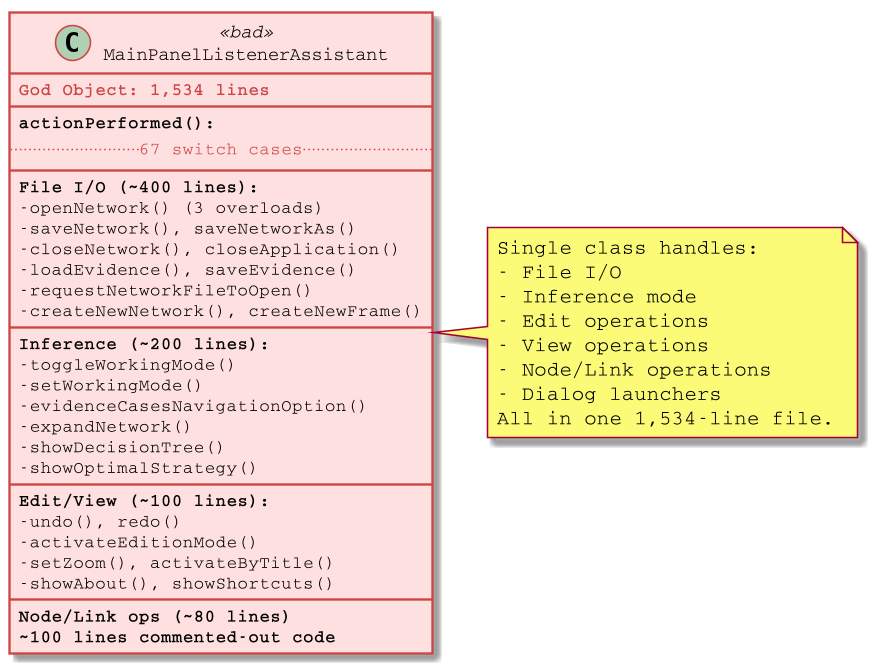
\includegraphics[width=0.65\textwidth]{r1-before.png}
\caption{Before R1: monolithic controller with 1,534~lines mixing
         five responsibilities.
         Diagram source: \file{r1-before.puml}.}
\label{fig:r1-before}
\end{figure}

Additionally, the class contained \textasciitilde100~lines of
commented-out dead code.

% -------------------------------------------------------------------
\subsection{After}
% -------------------------------------------------------------------

The class was decomposed into a thin facade plus three
domain-specific handlers:

\begin{figure}[H]
\centering
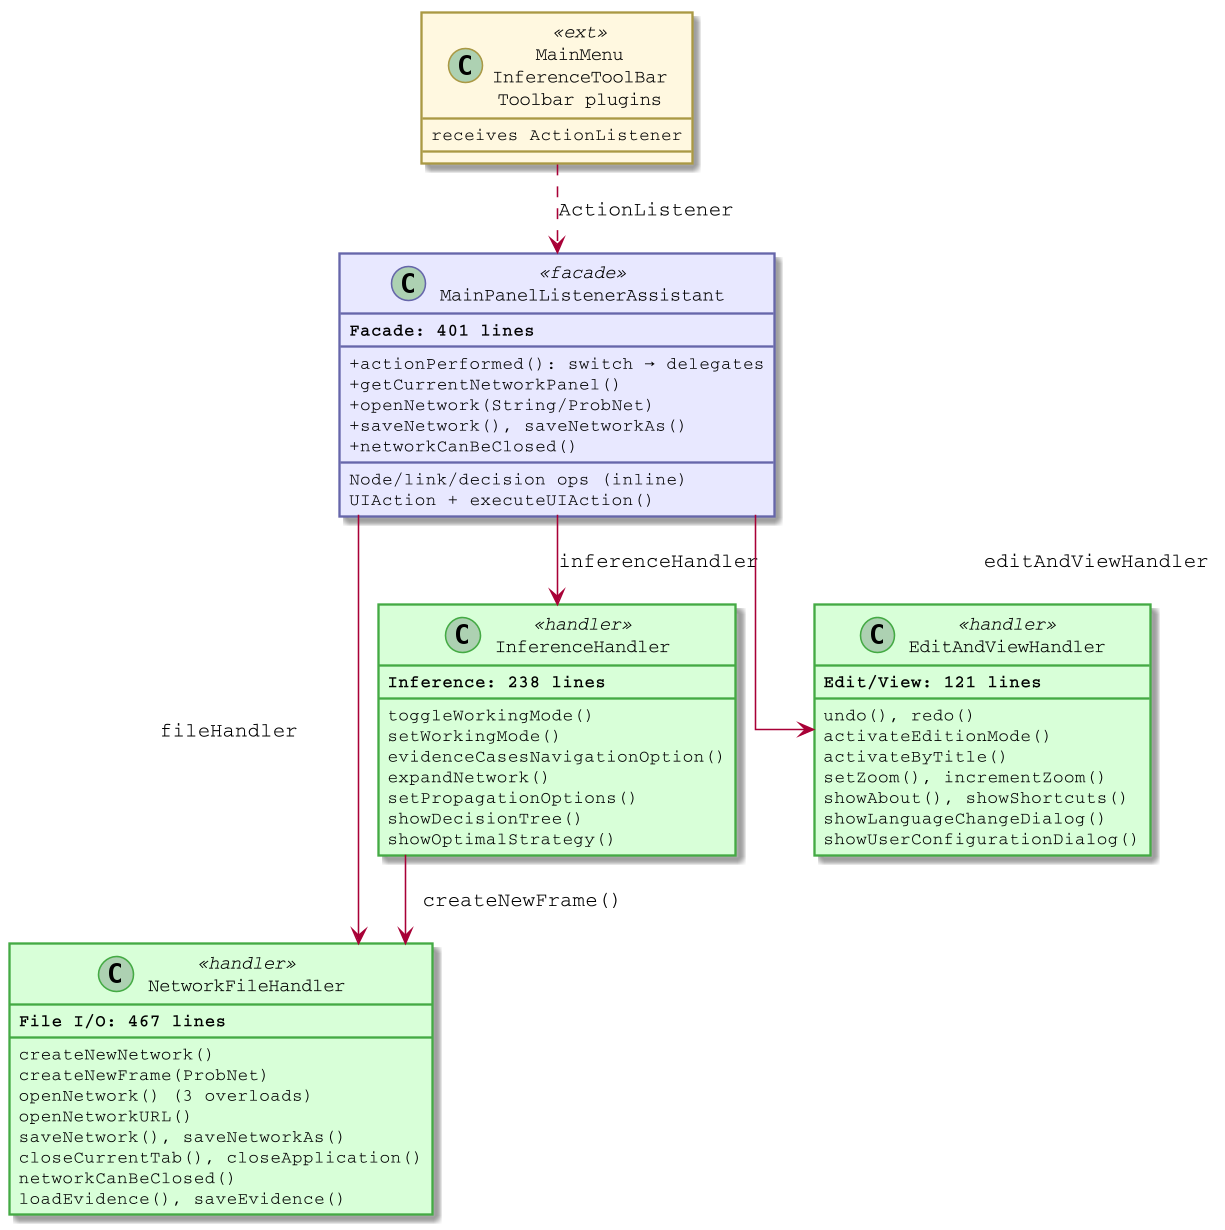
\includegraphics[width=0.95\textwidth]{r1-after.png}
\caption{After R1: facade delegates to three domain handlers.
         Diagram source: \file{r1-after.puml}.}
\label{fig:r1-after}
\end{figure}

\subsubsection{NetworkFileHandler (467 lines)}

All file I/O operations: open (3 overloads), save, save-as, close,
backup, evidence load/save, network creation, and file chooser
dialogs. This handler owns mutations to the shared
\code{networkPanels} list.

\subsubsection{InferenceHandler (238 lines)}

Inference mode switching, evidence case navigation, propagation and
inference options, network expansion, decision tree, and optimal
strategy display. Uses \code{NetworkFileHandler.createNewFrame()} for
the expand-network operation.

\subsubsection{EditAndViewHandler (121 lines)}

Undo/redo, edition mode activation, zoom, by-title/by-name toggle,
and dialog launchers (configuration, shortcuts, about, language
change).

\subsubsection{Facade (401 lines)}

\cls{MainPanelListenerAssistant} retains:
\begin{itemize}[nosep]
  \item \meth{actionPerformed()} --- the switch statement stays, but
        each case is a one-liner delegation to a handler.
  \item \code{UIAction} / \meth{executeUIAction()} --- the shared
        exception-wrapping pattern.
  \item Public API methods as thin delegates (\meth{getCurrentNetworkEditorPanel},
        \meth{openNetwork}, \meth{saveNetwork}, etc.).
  \item Inline node/link/decision operations (\textasciitilde80~lines)
        --- too scattered to justify a fourth handler.
  \item \code{WindowListener} and \code{ComponentListener} methods.
\end{itemize}

% -------------------------------------------------------------------
\subsection{Design rationale}
% -------------------------------------------------------------------

The handlers are \textbf{package-private} classes in
\code{org.openmarkov.gui.window}. No new public API is introduced.
External callers (9~modules, 35+ references to
\meth{getCurrentNetworkEditorPanel()}) are completely unaffected because
the facade preserves all public method signatures.

The \code{ActionListener} interface stays on the facade, so
\cls{MainMenu}, \cls{InferenceToolBar}, and toolbar plugins
(discovered via reflection in \cls{ToolbarManager}) continue to
receive the same \code{ActionListener} instance.

% -------------------------------------------------------------------
\subsection{Summary of impact}
% -------------------------------------------------------------------

\begin{table}[H]
\centering
\small
\begin{tabular}{lrl}
\toprule
\textbf{File} & \textbf{Lines} & \textbf{Role} \\
\midrule
MainPanelListenerAssistant (facade) & 401  & Event dispatch + public API \\
NetworkFileHandler                  & 467  & File I/O, open/save/close \\
InferenceHandler                    & 238  & Inference mode, evidence \\
EditAndViewHandler                  & 121  & Edit, view, dialogs \\
\midrule
\textbf{Total}                      & \textbf{1,227} & \\
\textbf{Original}                   & \textbf{1,534} & \\
\textbf{Net reduction}              & \textbf{$-$307 ($-$20\%)} & Dead code removed \\
\bottomrule
\end{tabular}
\caption{R1 impact: file sizes after decomposition.}
\label{tab:r1-impact}
\end{table}

The primary benefit is not line reduction but \textbf{separation of
concerns}: each handler has a single responsibility and can be
understood, tested, and modified independently.


% ===================================================================
\section{R7 --- VisualNetwork Decoupling from MainGUI}
\label{sec:r7}
% ===================================================================

\textbf{Files changed:} \file{graphic/VisualNetwork.java},
\file{window/edition/NetworkEditorPanel.java}

\subsection{Motivation}

\code{VisualNetwork} is a view-model class in the \code{graphic/} layer.
It implements \code{PNEditListener} to receive notifications when edits
are executed, undone, or redone on a \code{ProbNet}, and rebuilds the
visual representation accordingly.

However, it also held a \code{MainGUI} reference and used it to directly
enable/disable undo and redo toolbar buttons:

\begin{lstlisting}
mainGUI.mainPanel.getEditionToolBar()
    .getUndoButton().setEnabled(canUndo);
mainGUI.mainPanel.getEditionToolBar()
    .getRedoButton().setEnabled(canRedo);
\end{lstlisting}

This created \textbf{upward coupling}: a view-model class reached into
the UI layer (\code{MainGUI} $\to$ \code{MainPanel} $\to$
\code{EditionToolBar}) to toggle button state. This violates the
layered architecture and makes \code{VisualNetwork} harder to test and
reuse.

The same undo/redo button updates are already performed by
\code{MainPanelMenuAssistant}, which is also a \code{PNEditListener} on
the same \code{PNESupport}. Its \code{updateUndoRedo()} method calls
\code{setOptionEnabled(ActionCommands.UNDO, canUndo)} and
\code{setOptionEnabled(ActionCommands.REDO, canRedo)}.
The \code{setOptionEnabled()} method, inherited from \code{MenuAssistant},
iterates over all registered \code{MenuToolBarBasic} implementations ---
which include both \code{MainMenu} and the toolbar classes. Therefore, the
toolbar button updates in \code{VisualNetwork} were fully redundant.

\subsection{Before}

\begin{figure}[H]
\centering
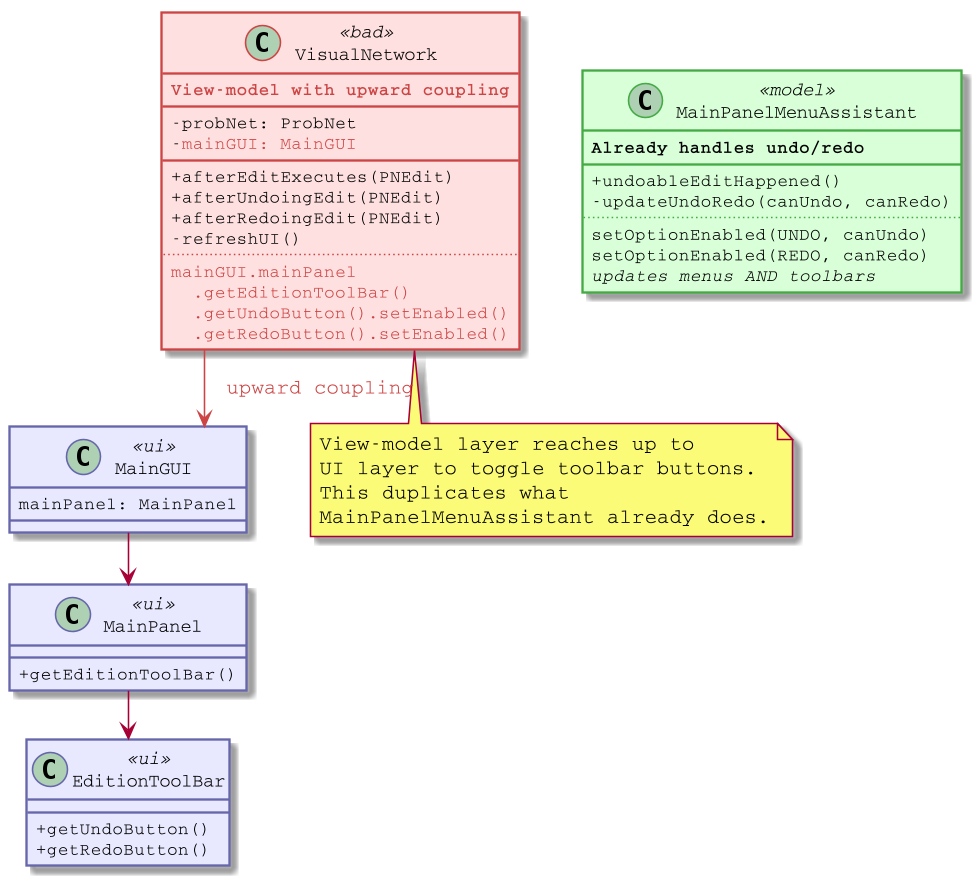
\includegraphics[width=0.85\textwidth]{diagrams/r7-before.png}
\caption{\code{VisualNetwork} coupled to \code{MainGUI} for undo/redo
         toolbar updates.}
\label{fig:r7-before}
\end{figure}

The \code{MainGUI} field was used in exactly 4 lines across two methods:

\begin{itemize}
  \item \code{afterEditExecutes(PNEdit)} --- lines 935--936
  \item \code{refreshUI()} (called by \code{afterUndoingEdit} and
        \code{afterRedoingEdit}) --- lines 976--978
\end{itemize}

\subsection{After}

\begin{figure}[H]
\centering
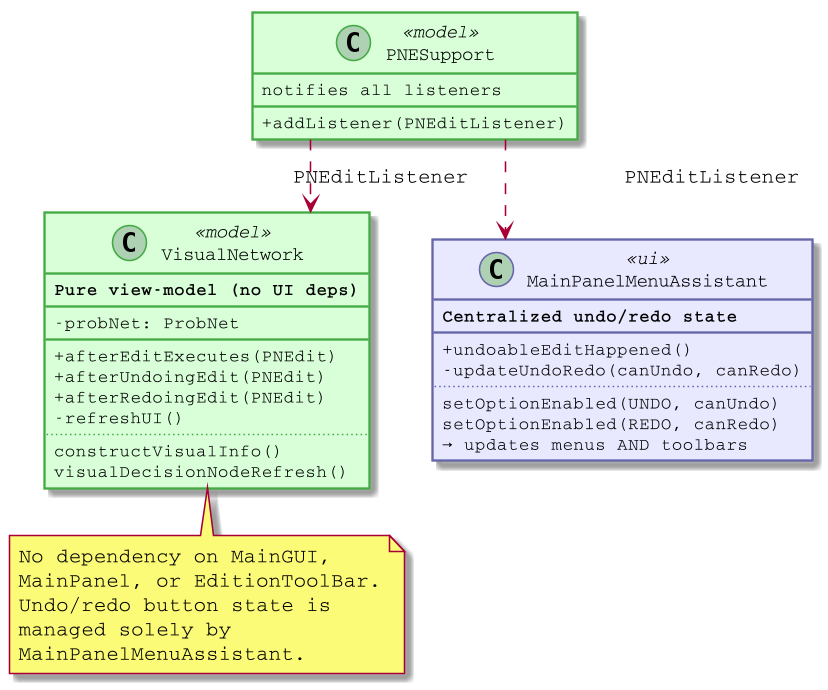
\includegraphics[width=0.85\textwidth]{diagrams/r7-after.png}
\caption{\code{VisualNetwork} decoupled: undo/redo state managed solely
         by \code{MainPanelMenuAssistant}.}
\label{fig:r7-after}
\end{figure}

Changes applied:

\begin{enumerate}
  \item Removed the \code{mainGUI} field from \code{VisualNetwork}.
  \item Removed the \code{MainGUI} parameter from the constructor
        (signature changed from \code{VisualNetwork(ProbNet, MainGUI)}
        to \code{VisualNetwork(ProbNet)}).
  \item Removed the 4 lines of direct toolbar button manipulation from
        \code{afterEditExecutes()} and \code{refreshUI()}.
  \item Removed the \code{MainGUI} import.
  \item Updated the single call site in \code{NetworkEditorPanel.java} to use
        the new one-argument constructor.
\end{enumerate}

\subsection{Summary of impact}

\begin{table}[H]
\centering
\begin{tabularx}{\textwidth}{l r r r X}
\toprule
\textbf{File} & \textbf{Before} & \textbf{After} & \textbf{$\Delta$} & \textbf{Change} \\
\midrule
\file{VisualNetwork.java} & 1{,}172 & 1{,}161 & $-$11 & Remove \code{mainGUI} field, constructor param, toolbar updates \\
\file{NetworkEditorPanel.java}  & ---     & ---     & $-$1  & Remove \code{mainGUI} argument from constructor call \\
\bottomrule
\end{tabularx}
\caption{R7 impact.}
\label{tab:r7-impact}
\end{table}

The line reduction is small, but the architectural benefit is significant:
\code{VisualNetwork} no longer depends on the UI layer and respects the
view-model boundary. The undo/redo button state is managed by a single
mechanism (\code{MainPanelMenuAssistant.setOptionEnabled()}), eliminating
redundancy and the risk of inconsistent updates.


% ===================================================================
\section{R6 --- ValuesTable Component Cleanup}
\label{sec:r6}
% ===================================================================

\textbf{Files changed:} 6 files in \file{component/} and
\file{dialog/link/}. One class deleted.

\subsection{Motivation}

The \file{component/} package contains a hierarchy of 10 classes
(4~table classes, 3~models, 6~renderers; 1,919 lines total) for editing
conditional probability tables (CPTs). After analysis, the subclass
overrides of \code{setValueAt()} and \code{afterEditExecutes()} represent
legitimate template method usage rather than fragile inheritance, and the
renderers implement genuinely different coloring logic. A full
consolidation would carry high regression risk for modest structural
benefit.

Instead, this refactoring focused on removing dead code, fixing a
shadowed field, and eliminating unused parameters --- concrete
improvements that reduce noise without touching the editing or rendering
logic.

\subsection{Changes}

\subsubsection{Deleted class: AugmentedValuesTableCellRenderer}

This renderer (32~lines) was never instantiated anywhere.
\code{AugmentedValuesTable} inherits its renderer setup from
\code{ValuesTable.defaultConfiguration()}, which sets
\code{ValuesTableCellRenderer} directly. The file was deleted.

\subsubsection{Dead code in AugmentedValuesTable}

Three methods removed:

\begin{itemize}
  \item \code{printTable()} (20~lines): Debug method overriding the
        parent's identically-named dead method. Neither version was
        ever called.
  \item \code{editCellAt()} override (8~lines): Called
        \code{super.editCellAt()} then added
        \code{System.err.println("CLICK COUNT...")}. Leftover debug
        code. Removing it lets the parent's version (which includes
        \code{selectAll()} for keyboard/mouse cell entry) apply
        correctly.
  \item \code{selectAll(EventObject)} (21~lines): Private method,
        never called. The parent's \code{editCellAt()} invokes the
        parent's own private \code{selectAll()} (Java resolves private
        methods at compile time). This copy was unreachable.
\end{itemize}

Six imports made unnecessary by these removals were also deleted.

\subsubsection{Dead code in ValuesTable}

\code{printTable()} (20~lines) removed --- debug method never called
from any code in the project.

\subsubsection{Shadowed field in ICIValuesTable}

\code{ICIValuesTable} declared \code{private int lastCol = -1}, which
shadows the parent's \code{protected int lastCol = -1}
(\file{ValuesTable.java}, line~152). Since the parent field is
\code{protected}, the subclass can access it directly. The shadow was
removed.

\subsubsection{Unused parameter in LinkRestrictionCellRenderer}

The constructor accepted a \code{TablePotential potential} parameter
that was never used. The parameter was removed from the signature, and
the 3 call sites in \code{LinkRestrictionPanel.setCellRenderers()} were
updated. The now-unnecessary \code{TablePotential} import was also
removed.

\subsubsection{Dead variable in LinkRestrictionValuesTable}

The constructor assigned \code{ProbNet net = node1.getProbNet()} but
never used \code{net}. The dead variable (and its source variable
\code{node1}) were removed, along with the unused \code{ProbNet} import.

\subsection{Summary of impact}

\begin{table}[H]
\centering
\begin{tabularx}{\textwidth}{l r r r X}
\toprule
\textbf{File} & \textbf{Before} & \textbf{After} & \textbf{$\Delta$} & \textbf{Change} \\
\midrule
\file{AugmentedValuesTableCellRenderer} & 32 & --- & $-$32 & Deleted (dead class) \\
\file{AugmentedValuesTable.java} & 267 & 183 & $-$84 & Dead methods + imports \\
\file{ValuesTable.java} & 873 & 852 & $-$21 & Dead \code{printTable()} \\
\file{ICIValuesTable.java} & 142 & 138 & $-$4 & Shadowed field \\
\file{LinkRestrictionCellRenderer.java} & 38 & 36 & $-$2 & Unused param \\
\file{LinkRestrictionValuesTable.java} & 109 & 100 & $-$9 & Dead variable + import \\
\midrule
\textbf{Total} & \textbf{1{,}461} & \textbf{1{,}309} & \textbf{$-$152} & \\
\bottomrule
\end{tabularx}
\caption{R6 impact: dead code removal and cleanup.}
\label{tab:r6-impact}
\end{table}

\subsection{What was not changed (and why)}

\begin{itemize}
  \item \textbf{Renderer consolidation}: The 5~remaining renderers
        implement genuinely different \code{setCellColors()} logic (ICI
        header coloring by parent variable, optimal policy
        max-detection, link restriction incompatibility coloring).
        Merging them into a single class would require a strategy
        pattern that adds complexity rather than reducing it.
  \item \textbf{PNEditListener extraction}: The listener callbacks
        (\code{afterEditExecutes}, \code{afterUndoingEdit}) are tightly
        coupled to the table's data model --- they call
        \code{getModel().setValueAt()} with specific row/column
        positions derived from edit objects. Separating them would
        require the controller to have intimate knowledge of the
        table's column and row structure.
  \item \textbf{Replacing inheritance with configuration}: Each
        subclass overrides \code{setValueAt()} and
        \code{afterEditExecutes()} with fundamentally different edit
        types (\code{TablePotentialValueEdit},
        \code{ICITablePotentialValueEdit},
        \code{AugmentedPotentialValueEdit},
        \code{LinkRestrictionPotentialValueEdit}). This is legitimate
        template method usage, not fragile inheritance.
\end{itemize}


% ===================================================================
\section{Verification}
\label{sec:verification}
% ===================================================================

All changes (R3, R5, R8, R4, R1, R7, R6) were verified by:

\begin{enumerate}
  \item Full compilation of all modules:
        \code{mvn install -DskipTests} --- \textbf{BUILD SUCCESS}
  \item GUI module tests:
        \code{mvn test -pl org.openmarkov.gui} ---
        \textbf{71 tests, 0 failures, 0 errors}
  \item Core module tests:
        \code{mvn test -pl org.openmarkov.core} ---
        \textbf{all passed}
\end{enumerate}

\end{document}
